\section{Аналитическая часть}

\subsection{Постановка задачи}\label{sec:task}
По заданию требуется разработать 


В соответствии с заданием необходимо разработать межсетевой экран, осуществляющий контроль проходящего сетевого трафика, в виде загружаемого модуля.

Необходимо предоставить пользователю возможность задания правил фильтрации пакетов и изменения видимости модуля в системе.

Для достижения поставленной цели необходимо решить следующие задачи:
\begin{enumerate}
	\item ознакомиться с основными принципами работы отдельных узлов распределённой системы и межсетевых экранов;
	
	\item ознакомиться со способом перехвата поступающих на хост пакетов;
	
	\item выбрать тип драйвера для перехвата входящих и исходящих пакетов;
	
	\item реализовать межсетевой экран. \newline
\end{enumerate}

\subsection{Передача информации}
В распределённых системах информация передаётся в виде пакетов по определёнными правилам -- протоколам. Каждый пакет проходит несколько стадий, которые определены в модели OSI (наглядно представлена в виде таблицы \ref{osi_table}) \cite{net}.

\begin{table}[h]
	\begin{center}
		\caption{Модель OSI}
		\label{osi_table}
		\begin{tabular}{| p{1cm} | p{7cm} |}
			\hline
			\textbf{№} 	& \textbf{Название} \\
			\hline
			7 				& Прикладной уровень\\ 
			\hline
			6 				& Уровень представления  \\ 
			\hline
			5 		& Сеансовый уровень \\ 
			\hline
			4 		& Транспортный уровень \\ 
			\hline
			3 		& Сетевой уровень \\ 
			\hline
			2 		& Канальный уровень \\ 
			\hline
			1 		& Физический уровень \\ 
			\hline
		\end{tabular}
	\end{center}
\end{table} 

\newpage

Из пакета можно получить информацию об IP-адресе источника/назначения, номере порта источника/назначения, протоколе и т.д. \newline

\subsection{Межсетевой экран}
\textbf{Межсетевой экран} -- это программное средство, предназначенное для фильтрации входящего и исходящего трафика, в соответствии с заранее заданными критериями, правилами, тем самым, осуществляя защиту компьютера от сетевых угроз. 

В общих чертах его работа изображена на Рисунке \ref{fig1:image}.

\begin{figure}[h]
	\centering
	\begin{center}
		{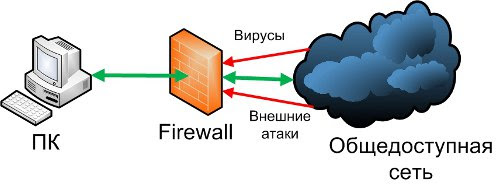
\includegraphics[scale=0.5]{img/firewall.jpg}}
		\caption{Принцип работы межсетевого экрана}
		\label{fig1:image}
	\end{center}
\end{figure}

\newpage

Межсетевой экран в основном работает на пакетном уровне (уровни 3 и 4 модели OSI, которая представлена в таблице \ref{osi_table}) \cite{fw}. 

Пакеты могут анализироваться по формальной корректности пакета, направлению (входящие/исходящие), типу протокола, порту (источника/назначения) и т.д. 

Для того, чтобы отфильтровать пакеты, пользователю необходимо задать соответствующие правила. Когда межсетевой экран перехватывает пакет, просматриваются его поля и сравниваются с существующими правилами, причём в том порядке, как они были заданы. Если совпадение было найдено, то пакет дальше не передаётся. \newline

\subsection{Загружаемые модули ядра}
Для того, чтобы добавить новые функции в ядро Linux, нужно либо перекомпилировать его (что небезопасно), либо воспользоваться загружаемым модулем ядра \cite{os}. 

После загрузки модуля он становится частью операционной системы и ему доступны все структуры и функции ядра. Когда функциональность, предоставляемая модулем, больше не требуется, то он может быть выгружен.

В Linux все модули обычно хранятся в каталоге /lib/modules и имеют расширение .ko. Модули загружаются и выгружаются с помощью специальных команд, приведённых в Листинге \ref{lst:module}.

\begin{lstlisting}[caption = {Команды для загрузки и выгрузки загружаемого модуля ядра}, label=lst:module]
insmod <имя модуля.ko>		// загрузить модуль в ядро
rmmod <имя модуля>			// выгрузить модуль из ядра
\end{lstlisting}

Загружаемый модуль ядра должен иметь определённую структуру. Обязательной частью любого загружаемого модуля являются:
\begin{itemize}
	\item функция загрузки (инициализации) модуля;
	
	\item функция выгрузки модуля; 
	
	\item макросы module\_init(init\_func), module\_exit(exit\_func);
	
	\item макрос MODULE\_LICENSE(char* license). \newline
\end{itemize}

\subsection{Изменение видимости модуля}
Для того, чтобы посмотреть все загруженные модули можно воспользоваться командой \textbf{lsmod}, которая читает /proc/modules и отображает информацию о файле в отформатированном списке \cite{lsmod}. 

Модуль описывается в системе с помощью структуры \textbf{struct module} (Листинг \ref{lst:struct_module}).
\begin{lstlisting}[caption = {struct module}, label=lst:struct_module]
	struct module
	{
		enum module_state state;
		struct list_head list; /* Member of list of modules */
		char name[MODULE_NAME_LEN]; /* Unique handle for this module */
		...
	};
\end{lstlisting}

В этой структуре поле list -- элемент связного списка модулей. При загрузке ядро добавляет модуль в список. При выгрузке, наоборот, исключает. 

Скрытие модуля подразумевает в себе задачу удаления соответствующего элемента из этого списка. А восстановление видимости, наоборот, добавление.

Для взаимодействия со списком модулей необходимо использовать структуру \textbf{struct list\_head} и функции \textbf{list\_add}, \textbf{list\_del}. Перед тем, как удалить модуль, следует сохранить указатель, чтобы можно было восстановить его видимость \cite{hide}.  \newline

\subsection{Управление внешними устройствами}
Поскольку принимается, что в Unix всё файл, устройства рассматриваются как специальные файлы, обеспечивающие связь между файловой системой и драйверами устройств. 

Для работы с ними используется структура \textbf{struct file\_operations} (Листинг \ref{lst:file_op}). 
\begin{lstlisting}[caption = {struct file\_operations}, label=lst:file_op]
struct file_operations {
	struct module *owner;
	...
	ssize_t (*read) (struct file *, char __user *, size_t, loff_t *);
	ssize_t (*write) (struct file *, const char __user *, size_t, loff_t *);
	...
	int (*open) (struct inode *, struct file *);
	...
	int (*release) (struct inode *, struct file *);
	...
}
\end{lstlisting}

Файлы устройств имеют три дополнительных атрибута, которые характеризуют устройство, соответствующее данному файлу:
\begin{enumerate}
	\item класс устройства;

	\item старший номер устройства, обозначающий его тип;
	
	\item младший номер устройства применяется для нумерации устройств одного типа.
\end{enumerate}

Для того, чтобы идентифицировать устройство, используются старший и младший номера \cite{os}.  \newline

\subsection{Анализ особенностей драйвера типа misc}
\textbf{Misc} (от слова "miscellaneous") \textbf{драйвером} называется простой символьный драйвер. Его используют в случаях, когда возможно использовать упрощение: не задавать самостоятельно старший номер устройства (major), поскольку он определён заранее и равен 10. Но разработчик должен задать младший номер в пределах от 1 до 255. \cite{2nd,misc}

Такой подход позволяет сэкономить оперативную память, особенно, если необходимо создать несколько символьных драйверов для нескольких простых устройств.

На misc драйверах могут быть определены операции open, read, write, close и т.д. И так же создаётся файл /dev/\{misc\_file\}.

По аналогии с символьными драйверами, которые описываются структурой struct cdev, для misc драйверов используется структура \textbf{struct miscdevice} (Листинг \ref{lst:misc}).
\begin{lstlisting}[caption = {struct miscdevice}, label=lst:misc]
struct miscdevice {
	int minor;
	const char *name;
	struct file_operations *fops;
	umode_t i_mode;
	struct miscdevice *next, *prev;
};
\end{lstlisting}

Поле minor может принимать значение MISC\_DYNAMIC\_MINOR, означающее, что оно будет определено автоматически \cite{3d}.

Для работы с таким драйвером используются функции, представленные в Листинге \ref{lst:misc_reg}.
\begin{lstlisting}[caption = {Функции для регистрации и удаления misc драйвера}, label=lst:misc_reg]
	int misc_register(struct miscdevice *misc);		// регистрация драйвера
	int misc_deregister(struct miscdevice *misc);	// удаление драйвера
\end{lstlisting}

\subsection{netfilter}
netfilter -- это механизм фильтрации сетевых пакетов, который позволяет отслеживать их перемещение и при необходимости можно перехватить, блокировать. \cite{hook} \newline

\subsubsection{Точки перехвата}
Путь сетевого пакета в ядре изображен на Рисунке \ref{fig2:image}. \\

\begin{figure}[ph!]
	\centering
	\begin{center}
		{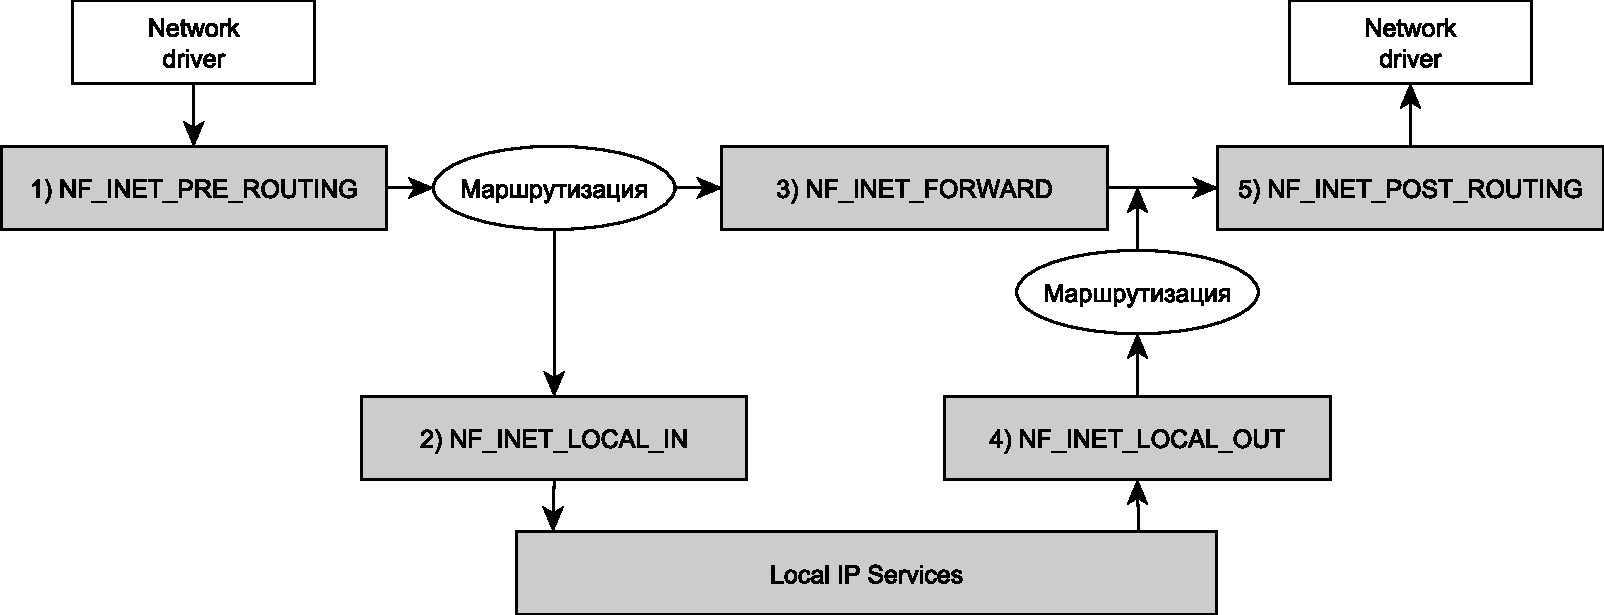
\includegraphics[scale=0.6]{img/packets.pdf}}
		\caption{Путь сетевого пакета}
		\label{fig2:image}
	\end{center}
\end{figure}

Предоставляется 5 точек, на которых могут быть определены функции перехвата, которые называются \textbf{хук-функциями}:
\begin{enumerate}
	\item NF\_INET\_PRE\_ROUTING – для всех входных пакетов;
	\item NF\_INET\_LOCAL\_IN – используется, чтобы перехватить пакеты, предназначенные для локального процесса;
	\item NF\_INET\_FORWARD – используется для пакетов, предназначенных для другого интерфейса;
	\item NF\_INET\_LOCAL\_OUT – для пакетов, которые создают локальные процессы;
	\item NF\_INET\_POST\_ROUTING – для пакетов, которые уже настроены для дальнейшего прохождения по сети к своему адресату и готовы покинуть текущий сетевой стек. \newline
\end{enumerate}

\subsubsection{Хук-функции}
Для того, чтобы использовать хук-функцию, необходимо сначала заполнить структуру \textbf{struct nf\_hook\_ops}. Структура с основными полями приведена в Листинге \ref{lst:hook}.

\begin{lstlisting}[caption = {struct nf\_hook\_ops}, label=lst:hook]
struct nf_hook_ops {
	nf_hookfn			*hook;
	...
	u_int8_t			pf;
	unsigned int		hooknum;
	int					priority;
};
\end{lstlisting}

В структуре находятся следующие поля:
\begin{itemize}
	\item \textbf{hook} -- функция, которая будет вызвана для обработки пакета, принимается решение отбросить или принять пакет;
	
	\item \textbf{pf} -- семейство протоколов;
	
	\item \textbf{hooknum} -- точка перехвата;
	
	\item \textbf{priority} -- приоритет. \\
\end{itemize}

Регистрация и удаление хуков осуществляется посредством вызова функций, которые представлены в Листинге \ref{lst:hook_reg}.

\begin{lstlisting}[caption = {Функции для регистрации и удаления хук-функций}, label=lst:hook_reg]
	// регистрация
	int nf_register_net_hook(struct net *net, const struct nf_hook_ops *ops);
	
	// удаление
	void nf_unregister_net_hook(struct net *net, const struct nf_hook_ops *ops);
\end{lstlisting}

\subsection{Выводы}
В этом разделе были сформулированы цель и задачи, рассмотрены основные этапы, также подробно изучены принципы работы межсетевого экрана. 

Для достижения поставленной цели было принято решение использовать простой misc драйвер, поскольку он ориентирован на выполнение небольших задач и имеет упрощённую схему создания.


 